\documentclass[11pt,a4paper]{article}
\usepackage[left=0.7in,right=0.7in,bottom=0.7in,top=0.7in]{geometry}

\usepackage[utf8]{inputenc}
\usepackage[english]{babel}
\usepackage{amsmath,bm}
\usepackage{graphicx}
\usepackage{colortbl}
\usepackage{xcolor}
\colorlet{lblue}{blue!50!black}
\usepackage[bookmarks=true,bookmarksnumbered=true,colorlinks=true,linkcolor=lblue,citecolor=lblue,urlcolor=lblue]{hyperref}
\usepackage{subfigure}
\usepackage{booktabs}
\RequirePackage{newtxtext,newtxmath}

\begin{document}
	
	

\section*{AE 6230 -- HW3: Mode Shapes and Responses of MDOF Systems}

\textbf{Out:} November 1, 2022; \textbf{Due:} November 8, 2022 by 11:59 PM ET in Canvas \\

\subsection*{Guidelines}

\begin{itemize}

    \item Read each question carefully before doing any work;

    \item If you find yourself doing pages of math, pause and consider if there is an easier approach;
	
    \item You can consult any relevant materials;
 
    \item You can discuss solution approaches with others, but your submission must be your own work;

    \item If you have doubts, please ask questions in class, during office hours, and/or Piazza (no questions via email);
	
    \item The solution to each question should concisely and clearly show the steps;

    \item Simplify your results as much as possible;

    \item Box the final answer for each question;        

    \item Submit any code with the solution (but remember to also submit all relevant plots).
	
\end{itemize}

\clearpage 

\subsection*{Problem 1 -- 40 points}

\begin{figure}[htpt!]
	\centering
	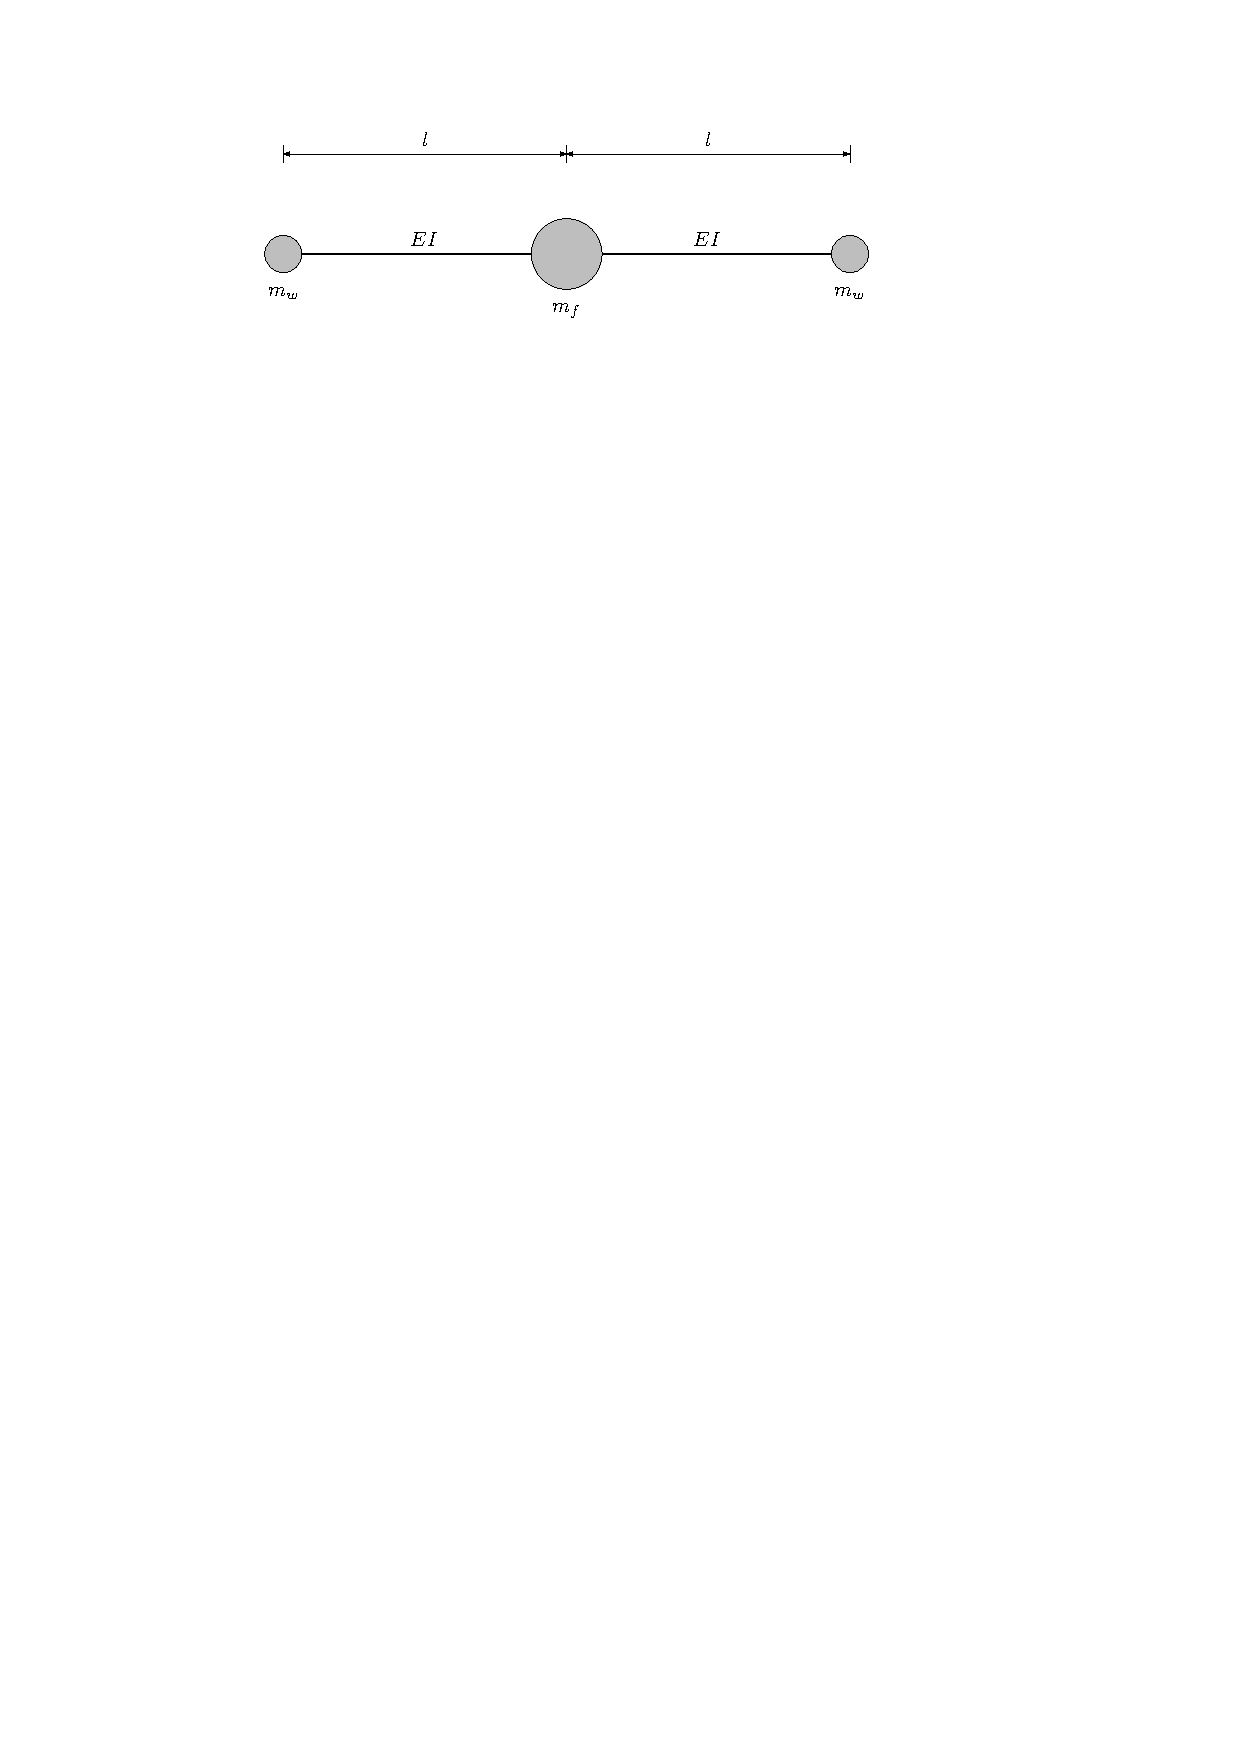
\includegraphics[width=0.6\textwidth]{figures/aircraft.pdf}
	\caption{Schematic of an aircraft undergoing out-of-plane (vertical) bending vibrations in free flight.}
	\label{f1}
\end{figure}
%
\begin{table}[htpt!]
	\centering
	\caption{Parameter values for Problem 1. \label{t1}}
	\vspace{2mm}
	\label{tab:1}
	\begin{tabular}{lrr}
		\toprule
		Parameter & Symbol & Value \\
		\midrule 
		Half-wing mass & $m_w$ & 750 kg \\
		Fuselage mass & $m_f$ & 5$m_w$ \\
		Wing semispan & $l$ & 10 m \\
		Wing out-of-plane bending stiffness & $EI$ & 5 $\times$ 10$^{6}$ Nm$^2$ \\
		\bottomrule
	\end{tabular}
\end{table}
%
Figure~\ref{f1} shows a simplified model for the out-of-plane (vertical) bending vibrations of a free-flying aircraft. The aircraft inertia is modeled by a concentrated mass $m_f$ at the fuselage centerline and two concentrated masses $m_w$ at the wing tips. The elasticity of each half wing is modeled by a beam of negligible mass with out-of-plane bending stiffness $EI$ and length $l$, which behaves as a spring $k = 3EI/l^3$. The aircraft motion is described in terms of the vertical translations of the left, center, and right masses, denoted by $h_{wl}(t)$, $h_{f}(t)$, and $h_{wr}(t)$, respectively. These translations are positive upward and measured from the undeformed configuration of the aircraft in Fig.~\ref{f1}. Assuming small-amplitude vibrations and neglecting gravity, answer the following questions:
%
\begin{enumerate}
	\item Considering the equations of motion 
	%
	\begin{equation} \label{e1}
		\begin{bmatrix}
			m_f & 0 & 0 \\
			0 & m_w & 0 \\
			0 & 0 & m_w 
		\end{bmatrix}
		\begin{Bmatrix}
			\ddot{h}_f \\
			\ddot{h}_{wl} \\
			\ddot{h}_{wr}
		\end{Bmatrix}
		+ 
		\frac{3EI}{l^3}
		\begin{bmatrix}
			2 & -1 & -1 \\
			-1 & 1 & 0 \\
			-1 & 0 & 1
		\end{bmatrix}
		\begin{Bmatrix}
			h_f \\
			h_{wl} \\
			h_{wr}			
		\end{Bmatrix}
		= 
		\begin{Bmatrix}
			0 \\
			0 \\
			0			
		\end{Bmatrix}
	\end{equation}
	%
	evaluate the natural frequencies for the parameters in Table~\ref{t1} (in ascending order);
	\item Evaluate the corresponding mode shapes normalized to have unit maximum displacement;
	\item Plot the mode shapes from Question 2 and interpret their meaning;
	\item Evaluate the inverse of the modal matrix $\mathbf{U}$ for the assumed mode shape normalization\footnote{Note that the assumed mode shape normalization yields non-unit modal mass.};
	\item Assuming that a wind gust causes the initial conditions
	%
	\begin{equation} \label{e2}
		\mathbf{q}(0) = \mathbf{q}_0 = 
		\begin{Bmatrix}
			0.5 \\ 
			0.0 \\
			0.0 \\
		\end{Bmatrix}
		\hspace{10mm}
		\dot{\mathbf{q}}(0) = \dot{\mathbf{q}}_0 = 0
	\end{equation}
	%
	determine the initial conditions for the modal equations;
	\item Write the analytical expression of the damped free response in the form
	%
	\begin{equation} \label{e3}
		\mathbf{q}(t) = \mathbf{U} \bm{\mathrm{\eta}}(t)
	\end{equation}
	%
	considering the modal viscous damping factors $\zeta_1 = 0, \zeta_2=\zeta_3 = 0.04$;
	\item Plot the components of $\mathbf{q}(t)$ and $\bm{\mathrm{\eta}}(t)$ for $0 \le t \le 20$ s;
	\item Explain the results from Question 7 (motivate the contribution from each mode).  
\end{enumerate}

\clearpage 

\subsection*{Problem 2 -- 30 points}

\begin{figure}[htpt!]
	\centering
	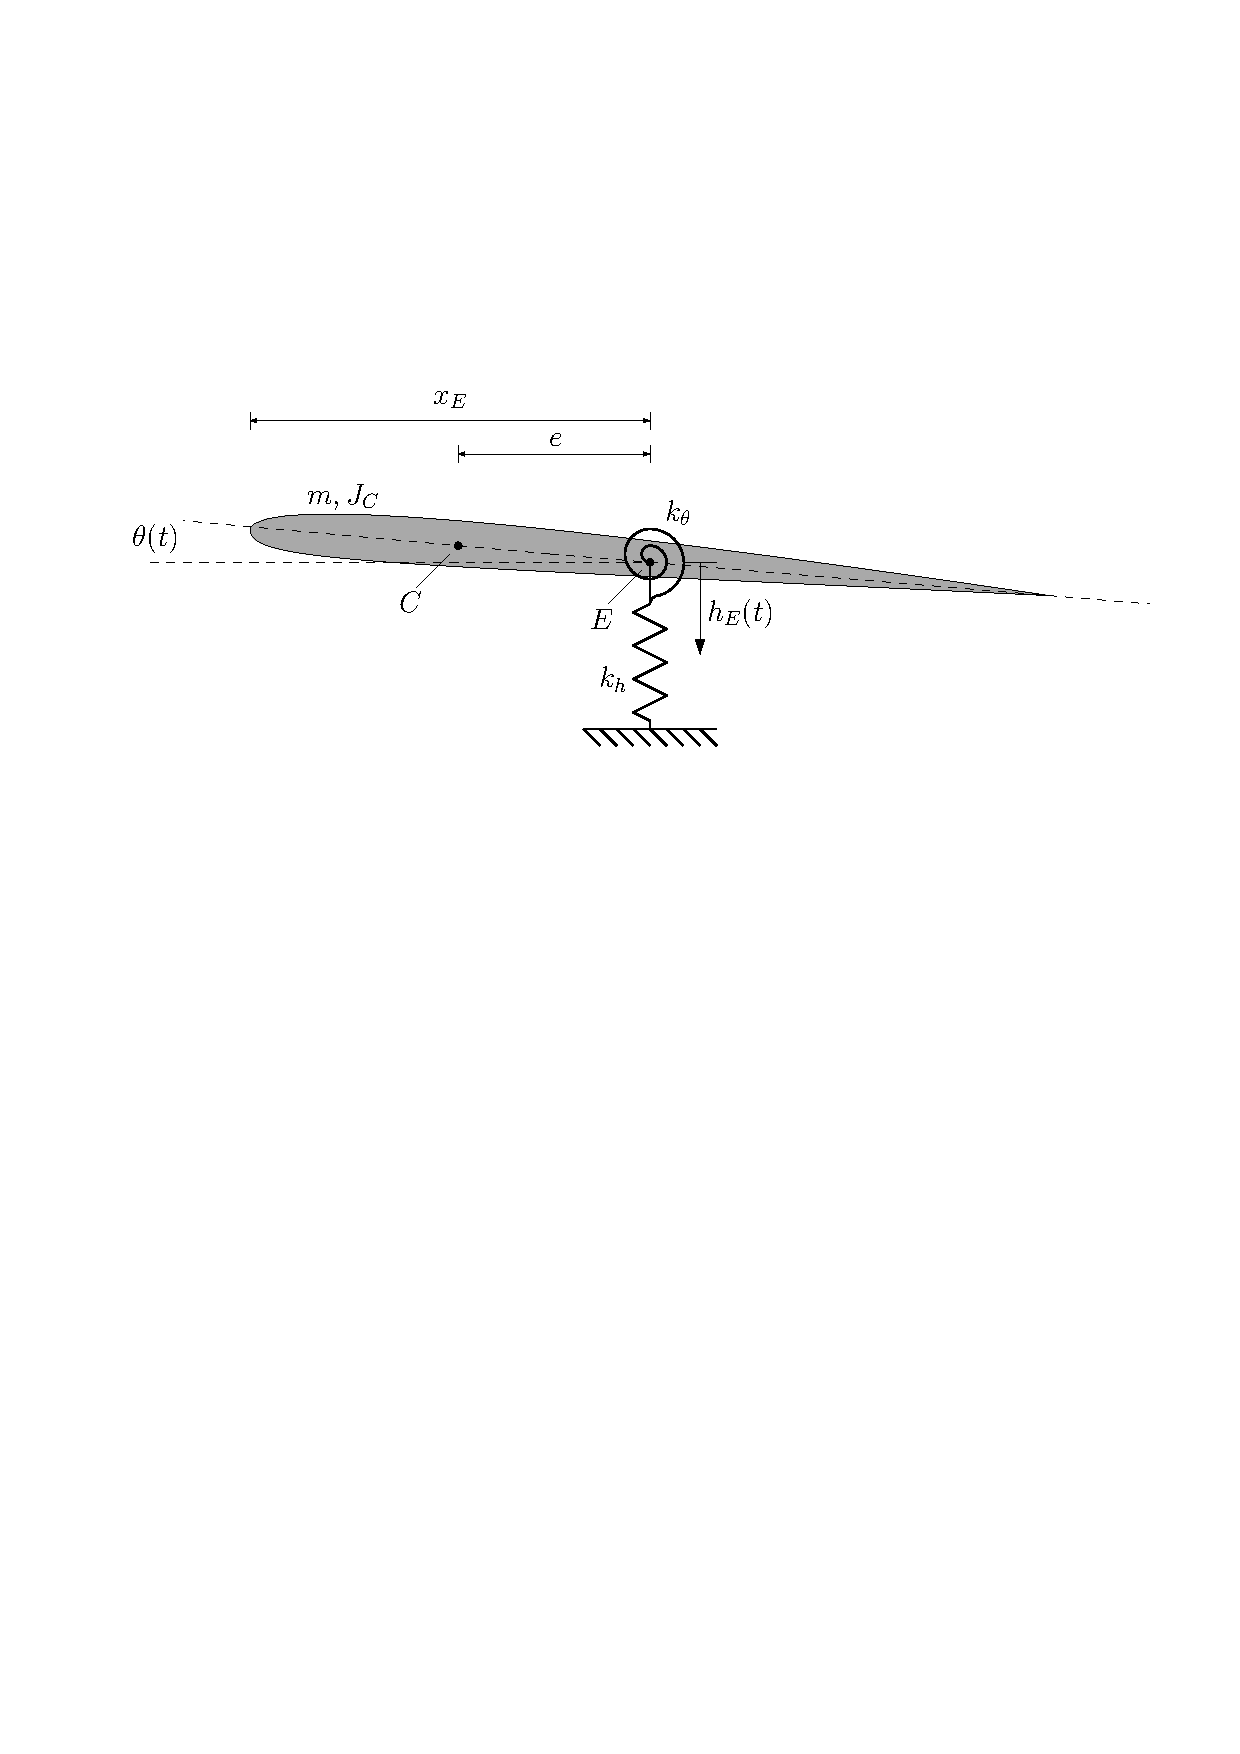
\includegraphics[width=0.9\textwidth]{figures/typical_section.pdf}
	\caption{Schematic of typical section model.}
	\label{f2}
\end{figure}
%
\begin{table}[htpt!]
	\centering
	\caption{Parameter values for Problem 2. \label{t2}}
	\vspace{2mm}
	\label{tab:2}
	\begin{tabular}{lrr}
		\toprule
		Parameter & Symbol & Value \\
		\midrule 
		Mass & $m$ & 10 kg \\
		Moment of inertia about $E$ & $J_E$ & 0.08 kg$\cdot$m$^2$ \\
		Chord & $c$ & 0.2 m \\
		Offset of $C$ from $E$ (positive as in Fig.~\ref{f2}) & $e$ & $-0.2c$ \\
		Position of $E$ along the chord (positive as in Fig.~\ref{f2}) & $x_E$ & 0.4$c$ \\
		Translational spring stiffness & $k_h$ & 1000 N/m \\
		Rotational spring stiffness & $k_\theta$ & 200 Nm/rad \\ 
		\bottomrule
	\end{tabular}
\end{table}
%
Consider the typical section model in Fig.~\ref{f2}, which is an abstraction for the cross section of a wing undergoing out-of-plane (vertical) bending and torsion. The typical section is subject to the excitation
%
\begin{equation}
	\mathbf{Q}(t) = 
	\mathbf{Q}_0
	\sin \omega_0 t
\end{equation}
%
with $Q_{0_1} = -10$ N, $Q_{0_2} = 1.5$ Nm, and $\omega_0 = 15$ rad/s. The modal mass and stiffness matrices along with the natural frequencies and mode shapes (normalized to have unit modal mass) can be computed using the script 
%
\begin{verbatim}
	AE6230_Fall2022_L17_MDOF_Free_TypicalSection.m	
\end{verbatim}
%
available in Canvas. Damping effects are captured by the modal viscous damping factors $\zeta_1 = \zeta_2 = 0.02$. Assuming small-amplitude vibrations and neglecting gravity, answer the following questions:
%
\begin{enumerate}
	\item Determine the modal excitation $\mathbf{N}(t)$;
	\item Considering the frequency response functions $H_1(\omega)$ and $H_2(\omega)$ associated with the modal coordinates $\bm{\mathrm{\eta}}(t)$
	%
	\begin{enumerate}
		\item Evaluate their magnitudes at the excitation frequency $\omega_0$;
		\item Evaluate their phase delays at that frequency;
	\end{enumerate}
	%
	\item Write the analytical expression of the damped steady-state response in the form of Eq.~\eqref{e3};
	\item Plot the components of $\mathbf{q}(t)$ and $\bm{\mathrm{\eta}}(t)$ for $0 \le t \le 2$ s;
	\item Explain the results from Question 4 (motivate the contribution from each mode).
	%
\end{enumerate}

\clearpage 

\subsection*{Problem 3 -- 30 points}

Consider the same typical section model as in Problem 2. The model experiences the step excitation
%
\begin{equation}
	\mathbf{Q}(t) = 
	\mathbf{Q}_0 \hspace{0.25mm}
	\mathrm{u}(t)
\end{equation}
%
with $Q_{0_1} = -10$, $Q_{0_2} = 1.5$ Nm, and zero initial conditions. Damping is captured by the proportional model
%
\begin{equation}
	\mathbf{C} = \alpha \mathbf{M} + \beta \mathbf{K}
\end{equation}
%
where $\alpha = 1.0$ s$^{-1}$ and $\beta = 1 \times 10^{-5}$ s. Answer the following questions:
%
\begin{enumerate}
	\item Evaluate the modal viscous damping factors $\zeta_1$ and $\zeta_2$;
	\item Evaluate the damped frequencies $\omega_{d_1}$ and $\omega_{d_2}$;
	\item Write the analytical expression of the damped response in the form of Eq.~\ref{e3};
	\item Plot the components of $\mathbf{q}(t)$ and $\bm{\mathrm{\eta}}(t)$ for $0 \le t \le 10$ s;
	\item Explain the results from Question 4 (motivate the contribution from each mode);
	\item Obtain the results from Question 4 for $e=-0.05c$ and explain any qualitative changes.
\end{enumerate}

\end{document}

